% !TEX root = ../main.tex
% \begin{center}
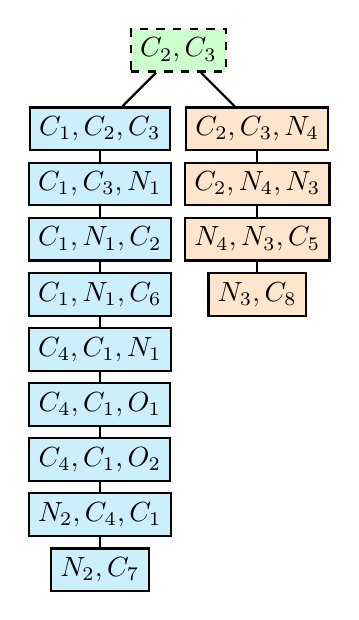
\begin{tikzpicture}[node distance={7mm}, thick, main/.style = {draw, rectangle}] 
\node[main, fill=green!20, dashed] at (0,0) (8) {$C_2,C_3$};
\node[main,fill=cyan!20] at (-1,-1) (7){$C_1,C_2,C_3$};
\node[main,fill=cyan!20] (100) [below of =7] {$C_1,C_3,N_1$};
\node[main,fill=cyan!20] (6) [below of =100]{$C_1,N_1,C_2$};
\node[main,fill=cyan!20] (5) [below of =6]{$C_1,N_1,C_6$};
\node[main,fill=cyan!20] (4) [below of =5]{$C_4,C_1,N_1$};
\node[main,fill=cyan!20] (3) [below of =4]{$C_4,C_1,O_1$};
\node[main,fill=cyan!20] (2) [below of =3]{$C_4,C_1,O_2$};
\node[main,fill=cyan!20] (1) [below of =2]{$N_2,C_4,C_1$};
\node[main,fill=cyan!20] (0) [below of =1] {$N_2,C_7$}; 

%\node[main,white] (00) [right = 1cm of 0] {}; 
%\node[main,white] (000) [left = 1cm of 0] {}; 



\node[main,fill=orange!20] at (1, -1) (9){$C_2,C_3,N_4$};
\node[main,fill=orange!20] (10) [below of =9]{$C_2,N_4,N_3$};
\node[main,fill=orange!20] (11) [below of =10]{$N_4,N_3,C_5$};
\node[main,fill=orange!20] (12) [below of =11]{$N_3, C_8$};


\draw [] (0) -- (1); 
\draw [] (1) -- (2); 
\draw [] (2) -- (3); 
\draw [] (3) -- (4); 
\draw [] (4) -- (5); 
\draw [] (5) -- (6); 
\draw [] (6) -- (100); 
\draw [] (7) -- (100); 
\draw [] (7) -- (8); 
\draw [] (8) -- (9); 
\draw [] (9) -- (10); 
\draw [] (10) -- (11); 
\draw [] (11) -- (12); 


\end{tikzpicture}
% \end{center}